\documentclass{standalone}

\usepackage{tikz}

\usepackage[T1]{fontenc}

\begin{document}
  \pagestyle{empty}

  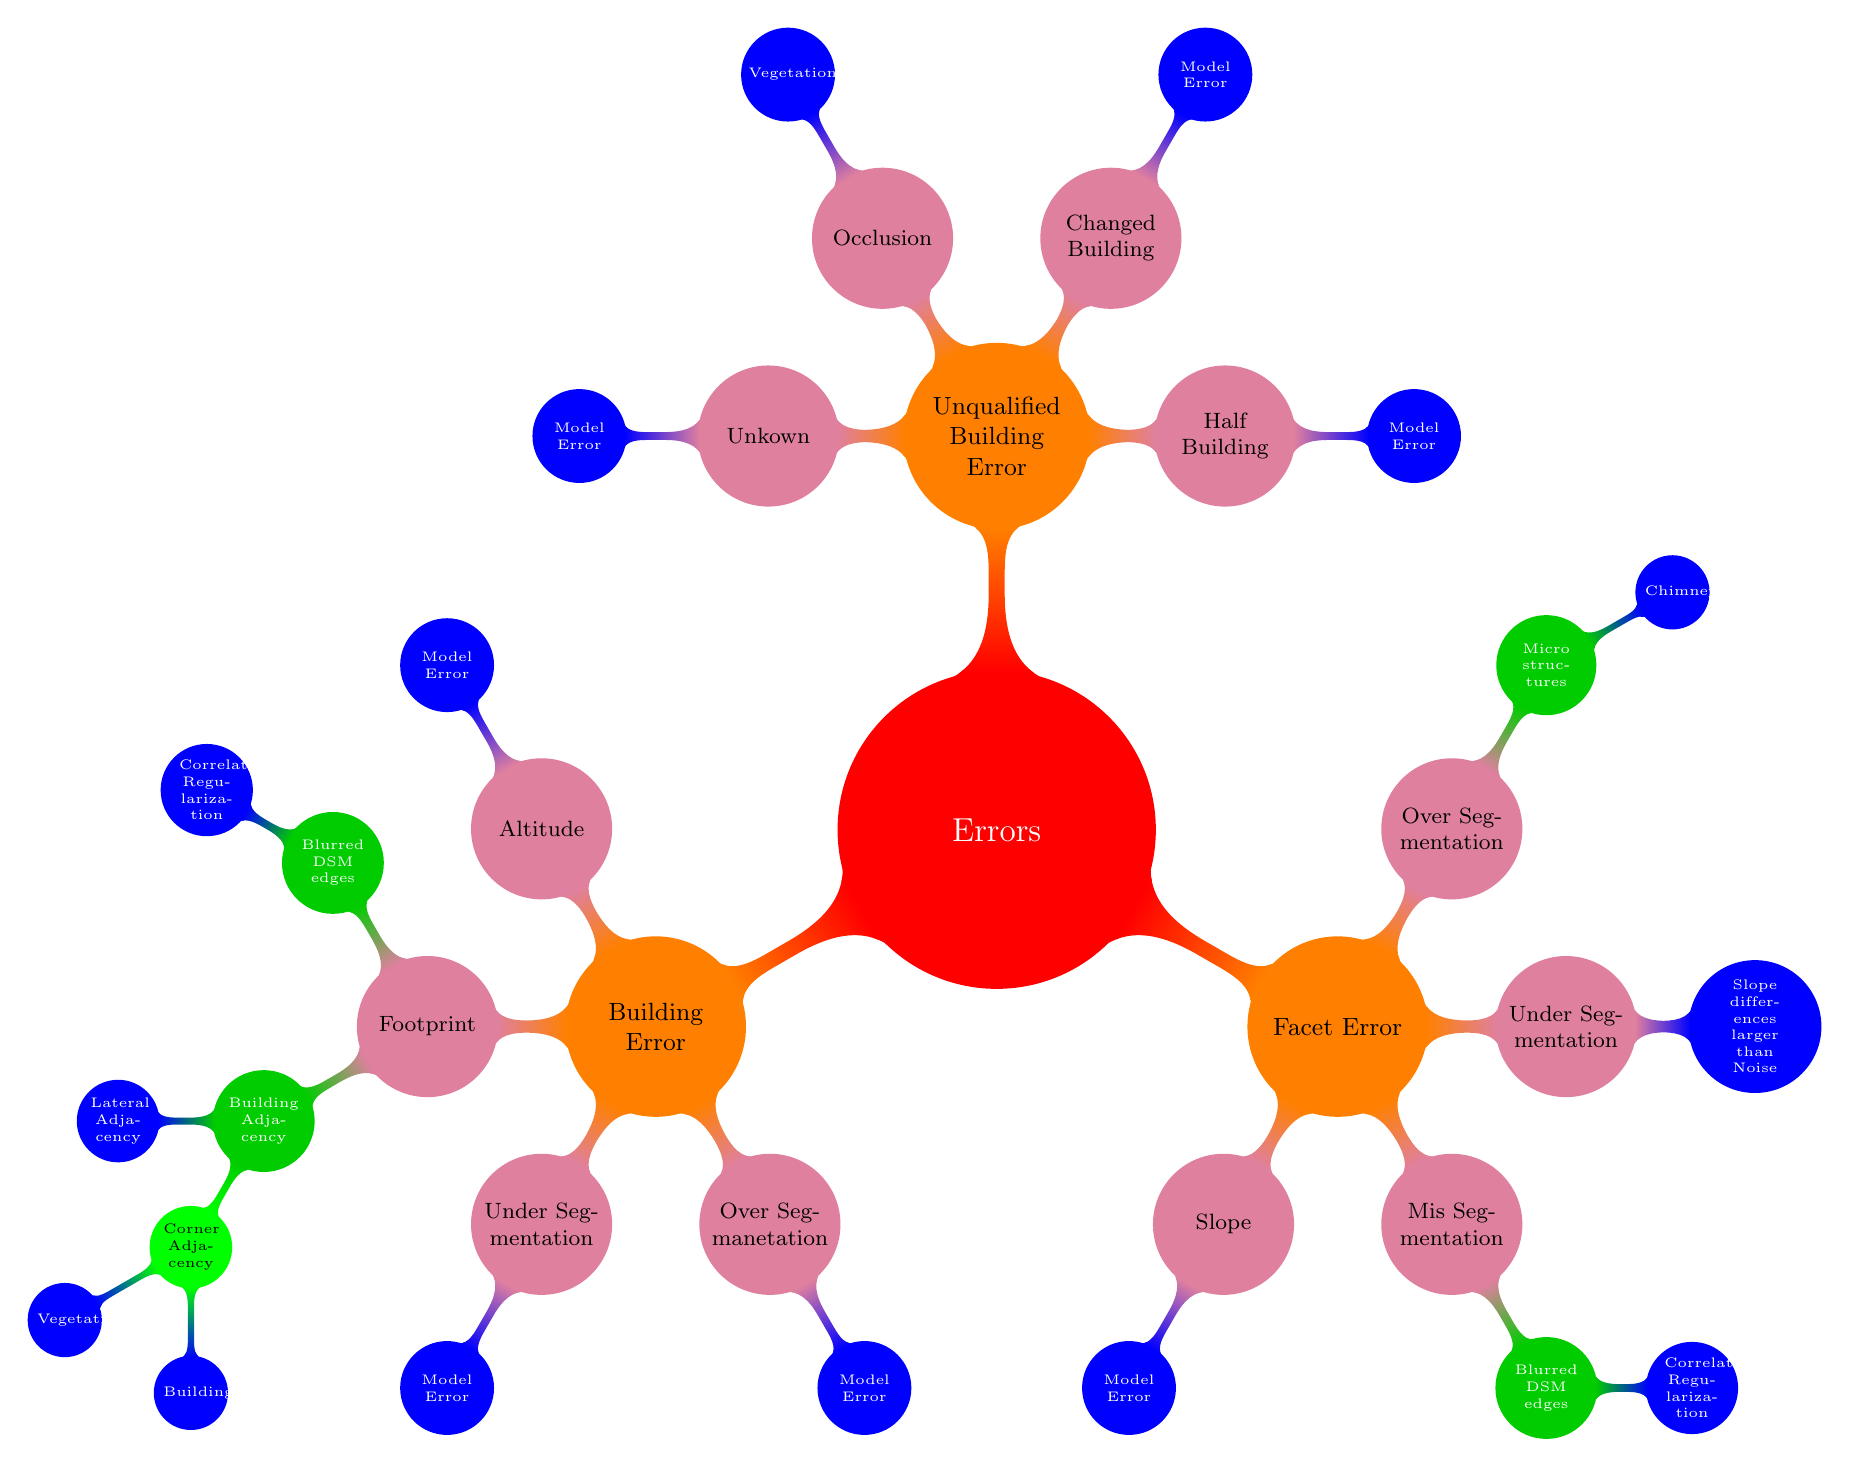
\begin{tikzpicture}
    \usetikzlibrary{mindmap, trees}
    \path[mindmap, concept color=red, text=white]
      node[concept]{Errors}[clockwise from=0]
      child[concept color=orange, text=black, grow=90]
      {
        node[concept]{Unqualified Building Error}[clockwise from=0]
        child[concept color=purple!50, text=black, grow=0]
        {
          node[concept]{Half Building}[clockwise from=0]
          child[concept color=blue, text=white, grow=0]
          {
            node[concept]{Model Error}
          }
        }
        child[concept color=purple!50, text=black, grow=60]
        {
          node[concept]{Changed Building}[clockwise from=0]
          child[concept color=blue, text=white, grow=60]
          {
            node[concept]{Model Error}
          }
        }
        child[concept color=purple!50, text=black, grow=120]
        {
          node[concept]{Occlusion}
          child[concept color=blue, text=white, grow=120]
          {
            node[concept]{Vegetation}
          }
        }
        child[concept color=purple!50, text=black, grow=180]
        {
          node[concept]{Unkown}
          child[concept color=blue, text=white, grow=180]
          {
            node[concept]{Model Error}
          }
        }
      }
      child[concept color=orange, text=black, grow=330]
      {
        node[concept]{Facet Error}
        child[concept color=purple!50, text=black, grow=60]
        {
          node[concept]{Over Segmentation}
          child[concept color=green!80!black, text=white, grow=60]
          {
            node[concept]{Micro structures}
            child[concept color=blue, text=white, grow=30]
            {
              node[concept]{Chimneys}
            }
          }
        }
        child[concept color=purple!50, text=black, grow=0]
        {
          node[concept]{Under Segmentation}
          child[concept color=blue, text=white, grow=0]
          {
            node[concept]{Slope differences larger than Noise}
          }
        }
        child[concept color=purple!50, text=black, grow=300]
        {
          node[concept]{Mis Segmentation}
          child[concept color=green!80!black, text=white, grow=300]
          {
            node[concept]{Blurred DSM edges}
            child[concept color=blue, text=white, grow=0]
            {
              node[concept]{Correlation Regularization}
            }
          }
        }
        child[concept color=purple!50, text=black, grow=240]
        {
          node[concept]{Slope}
          child[concept color=blue, text=white, grow=240]
          {
            node[concept]{Model Error}
          }
        }
      }
      child[concept color=orange, text=black, grow=210]
      {
        node[concept]{Building Error}
        child[concept color=purple!50, text=black, grow=300]
        {
          node[concept]{Over Segmanetation}
          child[concept color=blue, text=white, grow=300]
          {
            node[concept]{Model Error}
          }
        }
        child[concept color=purple!50, text=black, grow=240]
        {
          node[concept]{Under Segmentation}
          child[concept color=blue, text=white, grow=240]
          {
            node[concept]{Model Error}
          }
        }
        child[concept color=purple!50, text=black, grow=180]
        {
          node[concept]{Footprint}
          child[concept color=green!80!black, text=white, grow=120]
          {
            node[concept]{Blurred DSM edges}
            child[concept color=blue, text=white, grow=150]
            {
              node[concept]{Correlation Regularization}
            }
          }
          child[concept color=green!80!black, text=white, grow=210]
          {
            node[concept]{Building Adjacency}
            child[concept color=green, text=black, grow=240]
            {
              node[concept]{Corner Adjacency}
              child[concept color=blue, text=white, grow=210]
              {
                node[concept]{Vegetation}
              }
              child[concept color=blue, text=white, grow=270]
              {
                node[concept]{Building}
              }
            }
            child[concept color=blue, text=white, grow=180]
            {
              node[concept]{Lateral Adjacency}
            }
          }
        }
        child[concept color=purple!50, text=black, grow=120]
        {
          node[concept]{Altitude}
          child[concept color=blue, text=white, grow=120]
          {
            node[concept]{Model Error}
          }
        }
      };
  \end{tikzpicture}
\end{document}
